%filename Presentation-asclepiade
% ltex: language=fr
\documentclass[9pt]{bio_presentation}

% Per https://wwwnc.cdc.gov/eid/page/scientific-nomenclature:
% For organisms other than bacteria, fungi, and viruses, scientific names of taxa above the genus level (families, orders, etc.) should be in roman type.
\newcommand{\asclepias}{\textit{Asclepias}}
\newcommand{\lepidoptera}{Lepidoptera}
\newcommand{\plantae}{Plantae}

\newcommand{\asclepiassyriaca}{\textit{Asclepias syriaca}}
\newcommand{\asclepiasincarnata}{\textit{Asclepias incarnata}}
\newcommand{\arctiumlappa}{\textit{Arctium lappa}}
\newcommand{\solidagocanadensis}{\textit{Solidago canadensis}}

\newcommand{\danausplexippus}{\textit{Danaus plexippus}}
\newcommand{\limenitisarchippus}{\textit{Limenitis archippus}}

\author[Choulgian, Laforest, Landucci]{H.~Choulgian \and A.~Laforest \and N.~Landucci}
\title[Corrélation spatiale entre \asclepias\ et \danausplexippus]{Analyse de la corrélation spatiale entre les espèces du genre \asclepias\ et le papillon monarque (\danausplexippus) sur l'île de Montréal}
\institute[Collège Jean-de-Brébeuf]{Collège Jean-de-Brébeuf \\ Département de Biologie}
\date{11 novembre 2025}

\sloppy
\hyphenpenalty=999999
\addbibresource{monarques.bib}
\nocite{*}

\setbeameroption{show notes on second screen=right}

\newcommand{\graphic}[1]{%
    \begin{figure}[H]
        \rmfamily
        \small % Font size difference between Beamer and vanilla
        \resizebox{!}{0.8\textheight}{
            \input{#1.tikz}% compile script puts it on TEXPATH
        }
    \end{figure}
}

\newcommand{\photo}[3]{%
    \begin{figure}[H]
        \resizebox{!}{0.6\textheight}{
            \includegraphics{#1}% compile script puts it on TEXPATH
        }

        \small #2 \\ \scriptsize Crédit photographique: \cite{#3}
    \end{figure}
}

\newcommand{\kab}{K_{AB}(r)}
\newcommand{\normkab}{K_{AB}^*(r)}

\newcommand{\laxqty}[2]{\qty[parse-numbers=false]{#1}{#2}}
\newcommand{\noteqty}[2]{\qty[per-mode=fraction, forbid-literal-units=false]{#1}{#2}}

\def\colorize<#1>{\temporal<#1>{\color{black!60}}{\color{red}}{\color{black!40}}}

\begin{document}
\maketitle

\section{Contexte théorique}
\begin{frame}
    \frametitle{Question de recherche}
    \Large\bfseries Comment l'asclépiade (genre \asclepias) et le papillon monarque (\danausplexippus) sont-ils spatialement corrélés sur l'île de Montréal?

    \note{
        \large\bfseries Comment l'asclépiade (genre \asclepias) et le papillon monarque (\danausplexippus) sont-ils spatialement corrélés sur l'île de Montréal?
    }
\end{frame}
\begin{frame}
	\frametitle{Le papillon monarque (\danausplexippus)}
	\begin{columns}
		\begin{column}{0.5\textwidth}
			\photo{danaus_plexippus.jpg}{Papillon monarque adulte}{bressonComputerHotlineDanausPlexippus2009}
		\end{column}
		\begin{column}{0.5\textwidth}
			\photo{danaus_plexippus_caterpillar.jpg}{Chenille du papillon monarque}{ramseyMonarchButterflyDanaus2007}
		\end{column}
	\end{columns}

    \note{
        \begin{itemize}
            \item Espèce migratrice endémique d'Amérique du Nord
            \item Hiver: forêts sud USA~+ Mexique
            \item Depuis 1983, baisse de \qty{83}{\percent} de la surface occupée l'hiver au Mexique
            \item Au Canada, inscrit comme espèce en voie de disparition depuis décembre 2023
        \end{itemize}
    }
\end{frame}
\begin{frame}
	\frametitle{L'asclépiade (genre \asclepias)}
	\begin{columns}
		\begin{column}{0.5\textwidth}
            \photo{asclepias_syriaca.jpg}{Asclépiade commune (\asclepiassyriaca)}{doyleAsclepiasSyriacus2018}
		\end{column}
		\begin{column}{0.5\textwidth}
			\photo{asclepias_incarnata.jpg}{\asclepiasincarnata}{cbaile19AsclepiasIncarnataHomewood2024}
		\end{column}
	\end{columns}

    \note{
        \begin{itemize}
            \item Hôte obligatoire pour la chenille du monarque
            \item Jusqu'en 2014, considérée une mauvaise herbe nuisible
            \item À Montréal, \asclepiasincarnata\ beaucoup plus rare que l'asclépiade commune
        \end{itemize}
    }
\end{frame}
\begin{frame}
    \frametitle{L'île de Montréal}
    \begin{itemize}
        \item Présence d'îlots de chaleur
        \item Faible couvert végétal ($\sim \qty{7}{\percent}$ en superficie)
        \item Trame végétale éparse

    \end{itemize}

    \note{
        \begin{itemize}
            \item $\Delta$ de température affectent négativement le métabolisme du monarque (changements climatiques + îlots de chaleur)
            \item Couvert végétal $\approx \qty{7}{\percent}$, $\sim \qty{72}{\percent}$ de surfaces artificielles (Sud du Québec: $\sim \qty{72}{\percent}$ couvert végétal, $\sim \qty{2}{\percent}$ de surfaces artificielles
            \item Trame végétale éparse
            \item $\therefore$ différences dans la niche écologique du monarque en milieu urbain/rural
        \end{itemize}
    }
\end{frame}
\begin{frame}<1-11>
	\frametitle{La corrélation spatiale croisée}
    \onslide<1-3>{CSR: Complètement spatialement aléatoire (\textit{Completely spatially random})}
    \onslide<2->{
        \begin{columns}
            \begin{column}{0.4\textwidth}
                \begin{figure}[H]
                    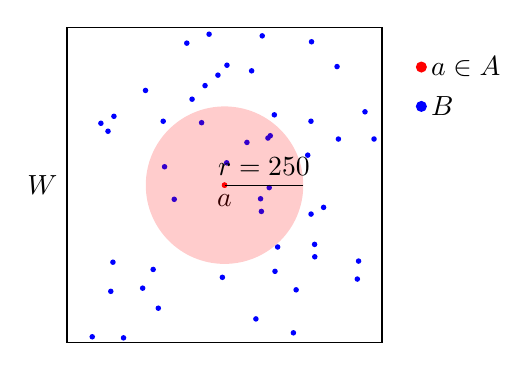
\begin{tikzpicture}
                        \pgfmathsetseed{6} % DO NOT CHANGE
                        \def\squaresize{2}
                        \def\margin{0.05}

                        \useasboundingbox (-\squaresize-0.5,-\squaresize) rectangle (\squaresize+1.5,\squaresize);
                        \draw (-\squaresize,-\squaresize) rectangle (\squaresize,\squaresize);

                        \foreach \i in {1,...,50} {
                            \fill<3->[blue] ({rand*(\squaresize-\margin)}, {rand*(\squaresize-\margin)}) circle (1pt);
                        }

                        \fill<5>[red] (0,0) circle (1pt) node[below, text=black] {$a$};
                        \fill<6->[red] (0,0) circle (1pt);
                        \fill<6->[red, opacity=0.2] (0,0) circle (\squaresize/2);
                        \draw<6-9> (0,0) -- (\squaresize/2,0) node[above, pos=0.5] {$r = \qty{250}{\m}$};

                        \node[left] at (-\squaresize, 0) {$W$};
                        \begin{scope}[shift={(\squaresize+0.5,\squaresize-0.5)}]
                            \fill<5->[red] (0,0) circle (2pt) node[right, text=black] {$a \in A$};
                            \fill<3->[blue] (0,-0.5) circle (2pt) node[right, text=black] {$B$};
                        \end{scope}
                    \end{tikzpicture}
                \end{figure}
            \end{column}
            \begin{column}{0.6\textwidth}
                \begin{itemize}
                    \only<1-4>{
                        \item<2-> $|W| = \qty{1}{\km\squared}$
                        \item<3-> $N_B = 50$
                        \item<4> $\lambda_B = \frac{N_B}{|W|} = \qty{50}{\per\km\squared}$
                    }
                    \only<5-8>{
                        \item<5-> $\lambda_B = \frac{N_B}{|W|} = \qty{50}{\per\km\squared}$
                        \item<7-> $n_B = \Bigl|\{b \in B | d(a,b) \le r\}\Bigr| = 10$
                        \item<8> $\kab = \frac{n_B}{\lambda_B} = \qty{0,2}{\km\squared}$
                    }
                    \only<9-10>{
                        \item<9> $\kab = \frac{n_B}{\lambda_B} = \qty{0,2}{\km\squared}$
                        \item<9> $\pi r^2 \approx \qty{0,196}{\km\squared}$
                        \item<10> CSR: $\kab \approx \pi r^2$
                    }
                    \only<11>{
                        \item CSR: $\kab \approx \pi r^2$
                        \item $\kab > \pi r^2$: $A$~attire~$B$
                        \item $\kab < \pi r^2$: $A$~repousse~$B$
                    }
                \end{itemize}
            \end{column}
        \end{columns}
    }

    \note{
        \begin{itemize}
            \only<1-5>{
                \item {\colorize<1> Position d'un pt: pas affectée par autres points}
                \item {\colorize<2> Prenons p.ex. zone d'étude~$W$, $\text{aire} = \qty{1}{\km\squared}$}
                \item {\colorize<3> Observation dans la zone: espèce~$B$, \num{50}~individus}
                \item {\colorize<4> $\therefore$ densité de pop. de \noteqty{50}{\text{individus}\per\km\squared}}
                \item {\colorize<5> On peut considérer un individu~$a$ de l'espèce~$A$ (point rouge).}
                \item {\colorize<6> Pour une échelle~$r$ donnée, on compte les points de~$B$ à une distance~$\le r$: ici,~$n_B = 10$} % just here for the shadow
            }
            \only<6->{
                \item {\colorize<6-7> Pour une échelle~$r$ donnée, on compte les points de~$B$ à une distance~$\le r$: ici,~$n_B = 10$}
                \item {\colorize<8> On calcule l'indice de Ripley bivarié~$\kab$ en divisant ce nombre d'individus par~$\lambda_B$, la densité de~$B$ à l'échelle de la densité de la zone d'étude}
                \item {\colorize<9> On peut aussi calculer l'aire du cercle de rayon~$r$: ici~$\text{aire} \approx \kab$}
                \item {\colorize<10> En général, si la distribution de~$B$ est aléatoire, $\kab \approx \pi r^2$}
                \item {\colorize<11> Similairement, si~$B$ est attiré ou repoussé par~$A$, $\kab \gtrless \pi r^2$}
                \item {\colorize<11> Dans le cadre de l'étude, on a calculé~$\kab$ pour différentes paires d'espèces, dont \danausplexippus, \asclepiassyriaca, \asclepiasincarnata, + 2 contrôles négatifs végétaux et 1 papillon contrôle négatif.}
            }
        \end{itemize}
    }
\end{frame}
\section{Résultats}
\begin{frame}
    \frametitle{Occurrences de diverses espèces végétales et de lépidoptères sur l'île de Montréal depuis 2020}
    \graphic{montreal_map}

    \note{
        Visuellement, \textit{clustering} observable dans plusieurs milieux verts:
        \begin{itemize}
            \item Forêt de Senneville
            \item Parc du Mont-Royal
            \item Parc-nature de la Pointe-aux-Prairies
        \end{itemize}
    }
\end{frame}
\begin{frame}
    \frametitle{Corrélation entre les espèces}
    \graphic{correlation}

    \note{
        Pour toutes les distances, corrélation $>$~CSR
    }
\end{frame}
\begin{frame}
    \frametitle{Corrélation normalisée entre les espèces $(r \ge \SI{50}{\m})$}
    \graphic{correlation_norm}

    \note{
        Ici, on a divisé~$\kab$ par~$\pi r^2$ (valeur attendue si CSR): on voit que~$> 1$ pour toutes les distances
    }
\end{frame}
\begin{frame}
    \frametitle{Corrélation normalisée entre les espèces $(\SI{50}{\m} \le r \le \SI{1}{\km})$}
    \graphic{correlation_close_norm}

    \note{
        \begin{itemize}
            \item Corrélation + plus forte à courte portée qu'à longue portée pour toutes les espèces
            \item Interaction entre asclépiade commune et monarque $>$~qu'avec les autres paires d'espèces (pour~$r < \qty{2,2}{\km}$)
        \end{itemize}
    }
\end{frame}

\section{Discussion}
\begin{frame}
    \frametitle{Interprétation des résultats}
    \begin{itemize}
        \item Rejet de l'hypothèse nulle~(CSR): $\kab > \pi r^2$ pour toutes les valeurs de~$r$
        \item Trame végétale urbaine~$\Rightarrow$ \textit{clustering} pour toutes les espèces
        \item Asclépiade et monarque: hôte obligatoire
    \end{itemize}

    \note{
        \begin{itemize}
            \item Facteurs expliquant une corrélation positive pour toutes les espèces
            \begin{itemize}
                \item On peut rejeter l'hypothèse nulle~(CSR): écart significatif entre le modèle de l'hypothèse nulle et les données expérimentales
                \item Trame urbaine: entraîne un \textit{clustering} d'une multitude d'espèces végétales et animales
            \end{itemize}
            \item Asclépiade et monarque: hôte obligatoire $\Rightarrow$ corrélation plus forte
            \begin{itemize}
                \item Le monarque ne peut pas vivre sans l'asclépiade
            \end{itemize}
        \end{itemize}
    }
\end{frame}
\begin{frame}
    \frametitle{Critique de l'étude}
    \begin{itemize}
        \item Observations biaisées?
            \begin{itemize}
                \item Naturalistes amateurs
            \end{itemize}
        \item Zone d'étude inadéquate
    \end{itemize}

    \note{
        \begin{itemize}
            \item Données utilisées viennent de naturalistes amateurs
                \begin{itemize}
                    \item Tendance à recenser des monarques là où des asclépiades sont présentes?
                    \item Solution: méthode des quadrats pour échantillonner partout
                \end{itemize}
            \item Zone d'étude utilisée (agglomération de Montréal) inclut des portions de cours d'eau et des surfaces artifielles (bétonnées)
                \begin{itemize}
                    \item Introduit des biais dans le calcul de~$\kab$
                    \item Solution: seulement considérer l'union de zones à haute valeur écologique
                \end{itemize}
        \end{itemize}
    }
\end{frame}

\printbibliography
\end{document}
